\documentclass[pdflatex,iicol,sn-mathphys-num]{sn-jnl}
\usepackage{graphicx}
\usepackage{amsmath,amssymb}
\usepackage{booktabs}
\raggedbottom
\begin{document}
\title[Same-parent consistency in \(^{129}\)Ba]{Same-parent consistency checks for the 365-keV transition in \(^{129}\mathrm{Ba}\)}
\author*[1]{\fnm{Author information} \sur{to be completed}}
\email{corresponding.author@to-be-completed}
\affil*[1]{\orgname{Affiliation and collaboration information to be completed}}

\abstract{The mixing ratio of the 365-keV transition in \(^{129}\mathrm{Ba}\) has been reconsidered in a proposed wobbling interpretation. We examine what its same-parent 461.6-keV companion can add to that inference. Specializing standard angular-distribution theory gives \(A_{4,t}=-(8/3)f_{E2}s_4A_{4,r}\), where \(f_{E2}=\delta^2/(1+\delta^2)\) and \(s_4\) is a finite-response ratio. This relation constrains a product; a calibrated response is required to infer the magnitude of \(\delta\). The evaluated central coefficients require a negative product, while a rank-2 check also has a central mismatch for equal responses. These observations motivate a fit in coefficient space rather than a division by a weak reference coefficient. Under a declared diagonal Gaussian covariance, the profiled distances for the small- and large-magnitude domains differ by only 0.0136. Their ordering changes within a specified covariance sensitivity family. A visually verified primary-table version has larger errors than the evaluation. With these errors, a nonnegative parent-population witness accommodates \(\delta=-2\) inside a two-margin box. The analysis identifies an unresolved companion-line consistency question, without assigning a new mixing ratio or a collective mode.}
\keywords{gamma-ray angular distribution, multipole mixing ratio, nuclear alignment, \(^{129}\)Ba}
\maketitle

\section{Physical question and existing method}

The electromagnetic character of interband transitions is important when testing wobbling interpretations in the \(A\approx130\) region. A quasiparticle--triaxial-rotor calculation relates spin-dependent energies to electromagnetic matrix elements, but an energy trend alone does not fix the transition operator or the experimental mixing ratio \cite{Frauendorf2014}. In \(^{129}\mathrm{Ba}\), Chakraborty et al. reexamined legacy angular-distribution coefficients and reported a minimum near \(\delta=-2\), with an approximately \(80(4)\%\) radiative \(E2\) fraction for the 365-keV line. They proposed a wobbling interpretation and requested further measurements \cite{Chakraborty2024}.

A useful reference already appears in the level scheme: the same \(13/2^-\) parent decays through the 364.7-keV mixed \(M1/E2\) line and a 461.6-keV line assigned \(E2\) \cite{Timar2014}. Can this companion independently constrain the branch choice? Using a pure transition from the same state to constrain alignment is an established technique, explicitly discussed by Diamond et al. \cite{Diamond1966}. The statistical-tensor and radiation-coefficient formalism is also standard \cite{Yamazaki1967,DerMateosian1974}. We make no claim to originate either principle. The present study applies them to a specific legacy-data consistency problem and examines the dependence on response and uncertainty assumptions.

A single rank-2 angular coefficient can admit two mixing-ratio magnitudes. A reliable rank-4 coefficient can distinguish them when alignment and response are known. With unknown alignment, even the two coefficients need not identify a unique magnitude. A same-parent reference is informative only if it samples the same selected parent ensemble and its multipolarity and response are established. These conditions are the subject of this study, rather than consequences of a level-scheme label.

\section{Source identity and numerical inputs}

We retain the evaluated ENSDF input in Table~\ref{tab:input}. The selected reaction dataset belongs to the 2014 \(A=129\) evaluation \cite{Timar2014}; it attributes the paired angular coefficients to Gizon et al. \cite{Gizon1977}. The two records share the 643.6-keV parent. The rounded 365-keV label is not used to match unrelated transitions.

\begin{table*}[t]
\centering
\caption{Separate evaluated and primary-publication inputs. Energies are in keV; quoted margins are preserved. These source versions share a historical lineage and are not pooled as independent measurements.}
\label{tab:input}
\begin{tabular}{@{}lccrr@{}}
\toprule
Line & \(J_i\to J_f\) & \(E_\gamma\) & \(A_2\) & \(A_4\)\\
\midrule
Mixed target & \(13/2^-\to11/2^-\) & 364.7 & \(-0.70(3)\) & \(+0.16(5)\)\\
\(E2\) reference candidate & \(13/2^-\to9/2^-\) & 461.6 & \(+0.22(2)\) & \(+0.08(5)\)\\
\midrule
1977 target & \(13/2^-\to11/2^-\) & 365.0 & \(-0.70(5)\) & \(+0.16(5)\)\\
1977 reference & \(13/2^-\to9/2^-\) & 461.8 & \(+0.22(4)\) & \(+0.08(6)\)\\
\bottomrule
\end{tabular}
\end{table*}

The complete 13-page Gizon et al. paper has now been obtained and its Table~1 visually checked \cite{Gizon1977}. It reports angular measurements at seven angles and Table~1 intensities at \(55^\circ\) to the beam. The 365.0- and 461.8-keV branches share a parent; later evaluated energies are retained as a separate version. The original table confirms both positive rank-4 coefficients.

The primary margins are 0.05 for the target \(A_2\) and 0.04/0.06 for the reference \(A_2/A_4\), compared with 0.03 and 0.02/0.05 in the evaluation. This is a verified difference between publications, not an OCR inference. Its origin in a later revision or evaluation procedure remains unresolved because the 1978 polarization article has not been acquired in full. Each dataset is analyzed separately. No original angular yields or numerical covariance have been recovered.

\section{Same-parent angular constraints}

For an axially aligned ensemble and a response that permits scalar angular-rank folding, write
\begin{equation}
 A_{k,x}=\rho_{k,x}Q_{k,x}F_{k,x}(\delta_x),\qquad x=t,r.
\end{equation}
Here \(\rho_k\) describes nuclear alignment, \(Q_k\) the finite response, and \(F_k\) the radiation coefficient in a specified phase convention. Shared selected-parent populations imply \(\rho_{k,t}=\rho_{k,r}\). Different gates or time selections may violate this equality even when the state identity agrees.

For an \(M1/E2\) target, the rank-4 \(M1/M1\) and interference terms vanish by angular-momentum coupling. A pure-\(E2\) reference consequently gives
\begin{equation}
 \begin{aligned}
 A_{4,t}&=-\frac83 f_{E2}s_4 A_{4,r},\\
 f_{E2}&=\frac{\delta^2}{1+\delta^2},\qquad
 s_4=\frac{Q_{4,t}}{Q_{4,r}}.
 \end{aligned}
 \label{eq:rank4}
\end{equation}
The signed radiation factors for this spin sequence are
\begin{equation}
 F_{4,t}=\frac{32\sqrt{2431}}{3003},\qquad
 F_{4,r}=-\frac{4\sqrt{2431}}{1001}.
\end{equation}
Their ratio is \(-8/3\). An exact factorial calculation and an independent standard Wigner-symbol calculation agree. Direct photon-amplitude projections for all 14 parent magnetic substates also verify the cancellation for common diagonal populations; no Gaussian alignment assumption is needed.

Equation~\eqref{eq:rank4} identifies only \(f_{E2}s_4\) when \(s_4\) is unknown. With a known nonzero \(s_4\), the allowed \(f_{E2}\) determines \(\lvert\delta\rvert\), but \(f_{E2}(\delta)=f_{E2}(-\delta)\) leaves the sign undetermined. If the reference coefficient vanishes, ratio inversion is undefined. A known negative \(s_4\) is mathematically usable; nonnegative detector efficiency does not by itself guarantee a positive rank-4 attenuation factor.

For different selected-parent populations a separate factor \(g_4=\rho_{4,t}/\rho_{4,r}\) remains in Eq.~\eqref{eq:rank4}. It is not an instrumental \(Q_4\). Reference multipole contamination changes the radiation coefficient, while a general angular response can mix ranks and require a fuller treatment. These effects cannot all be absorbed into a negative \(s_4\).

The rank-2 companion relation supplies a second check on the same observations. In the declared phase convention,
\begin{equation}
 \frac{A_{2,t}}{A_{2,r}}=s_2 q(\delta),\qquad
 q(\delta)=\frac{-7+14\sqrt{11}\delta-\delta^2}{10(1+\delta^2)}.
 \label{eq:rank2}
\end{equation}
Its two-dimensional quadratic-form eigenvalues give the exact range
\begin{equation}
 \frac{-2-\sqrt{137}}5\le q(\delta)\le
 \frac{-2+\sqrt{137}}5.
\end{equation}
The central ratio \(-0.70/0.22=-3.1818\) is below the lower limit \(-2.74094\) for \(s_2=1\). Allowing a positive \(s_2\) requires at least 1.16085 at these central values. This amplitude check needs a response magnitude, whereas the rank-4 opposite-sign condition needs only \(s_4>0\). Neither is a statistical rejection of noisy data.

\section{Profiling the original coefficients}

The reference \(A_4\) is only 1.6 times its evaluated margin. Rather than approximate its ratio as Gaussian, we work with
\(y=(A_{2,t},A_{4,t},A_{2,r},A_{4,r})^T\).
For fixed \(\delta,s_2,s_4\), let \(c_2=s_2q(\delta)\),
\(c_4=-\tfrac83s_4f_{E2}\) and
\begin{equation}
 B_\delta=\begin{pmatrix}c_2&0\\0&c_4\\1&0\\0&1\end{pmatrix}.
\end{equation}
The unknown true reference coefficients form \(b=(b_2,b_4)^T\). For a fixed positive-definite Gaussian covariance \(V\), the profiled residual distance is
\begin{align}
 D(\delta)&=\min_b(y-B_\delta b)^T V^{-1}(y-B_\delta b)\\
 &= (L_\delta y)^T(L_\delta V L_\delta^T)^{-1}(L_\delta y),
 \label{eq:profile}\\
 L_\delta&=\begin{pmatrix}1&0&-c_2&0\\0&1&0&-c_4\end{pmatrix}.
\end{align}
This is Gaussian nuisance profiling with fixed \(V\), not marginalization; no determinant of the projected covariance is added. Allowing any real \(b\) relaxes physical population-positivity constraints, so a fit does not certify a realizable alignment distribution.

We use \(s_2=s_4=1\) as a diagnostic scenario. With the four quoted margins collected in \(S\), the covariance sensitivity family is
\begin{equation}
 V=S\,[R(\rho_c)\otimes R(\rho_w)]\,S,
 \qquad R(\rho)=\begin{pmatrix}1&\rho\\\rho&1\end{pmatrix}.
\end{equation}
Here \(\rho_w\) couples angular ranks within each line and \(\rho_c\) couples lines. We scan each over \(-0.8,-0.4,0,0.4,0.8\); these are chosen correlations, not measured values or an exhaustive covariance model. Minimization uses \(\theta=\arctan\delta\), with the pure-\(E2\) endpoints included. Small- and large-magnitude domains share the \(\lvert\delta\rvert=1\) boundary in their closures. Distances and contrasts receive no p-value, confidence-interval or branch-probability interpretation.

\section{Results and sensitivity}

The rank-4 central coefficients give \(f_{E2}s_4=-0.75\). For \(s_4>0\), their same signs cannot be exact means under the shared-parent and pure-reference assumptions. Their one-margin boxes are also both positive. However, the illustrative two-margin comparison at \(s_4=1\) is fragile: the evaluated reference box maps to an upper target value 0.0533, just below the target lower value 0.06. Raising \(s_4\) to 1.125 permits contact. Using the primary-table reference margin 0.06 gives an upper image of 0.1067 and hence overlap. These are literal marginal boxes, not joint confidence regions.

A further existence check enforces a physical aligned density: \(q_m=P(m)+P(-m)\ge0\), \(\sum_{m>0}q_m=1\), for the seven parent substate pairs. At a chosen \(\delta\), the four coefficients are linear in \(q_m\). Linear programming minimizes a common margin multiplier \(t\), subject to \(\lvert\mu_i(q)-y_i\rvert\le t s_i\), with unit response and a pure reference. For \(\delta=-2\), the optimum is 1.85768 for the primary data and 3.39629 for the evaluation. Thus a positive-density witness exists inside the primary two-margin box. Its weights are not a measured alignment distribution; the test neither assigns confidence coverage nor determines which populations the reaction actually produces.

\begin{table}[t]
\centering
\caption{Conditional diagonal-covariance results with \(s_2=s_4=1\). The minimizers describe the diagnostic; they are not revised experimental mixing ratios.}
\label{tab:results}
\small
\begin{tabular}{@{}lrr@{}}
\toprule
Quantity & Evaluated & Primary 1977\\
\midrule
\(\delta\) at minimum & \(-1.0270\) & \(-1.2412\)\\
\(D_{\min}\) & 12.8797 & 8.2357\\
\(D_{\rm small}-D_{\rm large}\) & 0.0136 & 0.4685\\
\bottomrule
\end{tabular}
\end{table}

The joint coefficient calculation in Table~\ref{tab:results} does not provide a stable large-versus-small distinction. For evaluated margins and \(\rho_c=0\), varying \(\rho_w\) from \(-0.8\) to \(+0.8\) changes \(D_{\rm small}-D_{\rm large}\) from \(+3.530\) to \(-1.931\). The ordering thus reverses inside this specified family. The primary-table calculation changes the distances again (Fig.~\ref{fig:profiles}). None of these assumed covariances has been established for the source experiment. The calculation demonstrates dependence on missing inputs, rather than measuring the correct covariance or reproducing the 2024 fit.

\begin{figure*}[t]
\centering
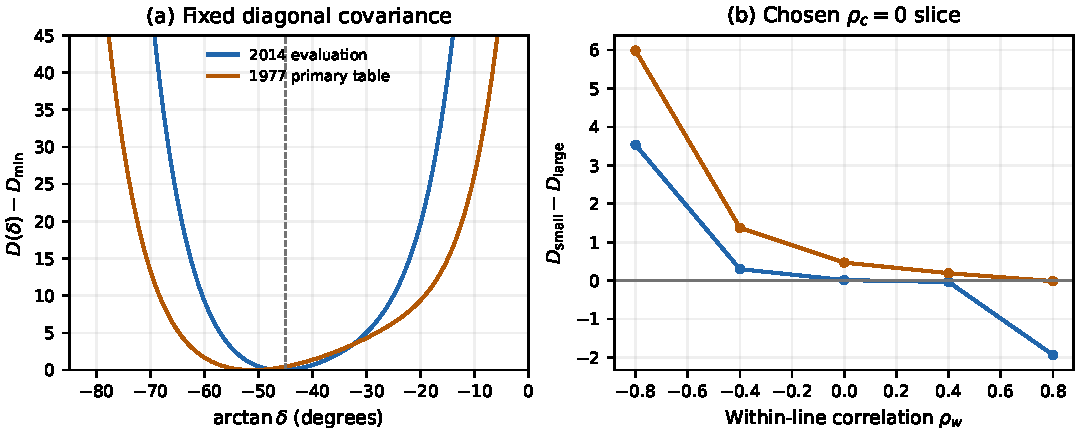
\includegraphics[width=0.88\textwidth]{figures/companion_profiles.pdf}
\caption{Declared two-rank coefficient-space diagnostics. (a) Profile distance above each diagonal-covariance minimum; the dashed line is \(\lvert\delta\rvert=1\). (b) Small-minus-large domain distance along the chosen \(\rho_c=0\) slice. The two curves retain the same evaluated means and signs but use different error scales. No line represents a statistical rejection threshold.}
\label{fig:profiles}
\end{figure*}

Numerical checks compare Eq.~\eqref{eq:profile} with a direct whitened least-squares fit, agreeing within \(1.2\times10^{-12}\). Doubling the angular search grid from 1025 to 2049 points before refinement changes the diagonal minima by less than \(9\times10^{-15}\). An isotropic zero-reference control has no \(\delta\) sensitivity, as required. These checks establish implementation consistency, not experimental coverage. Coverage would require repeated sampling under a justified observation model.

\section{Implications}

The same-parent line is useful because it adds a falsifiable consistency requirement to a mixing-ratio analysis. It has not yet supplied a new experimental root. Resolving the \(^{129}\mathrm{Ba}\) case requires resolving the later uncertainty revision and establishing the response ratio, reference purity, and joint fit or calibration covariance. The original table itself is now visually verified. The primary source's discussion of single-spectrum angular measurements narrows the experimental question; speculative gate differences cannot substitute for evidence about that acquisition.

The 2024 paper reports a joint angular-coefficient minimum. Our additional companion-reference assumptions are not a reconstruction of its fitting procedure, and the present results do not establish why its branch differs from historical values. Electromagnetic fractions also do not fix absolute collectivity: lifetime and branching information would still be required for an absolute \(B(E2)\) test. The analysis therefore leaves wobbling, signature-partner and tilted-precession interpretations to comparisons with complete electromagnetic evidence.

\section{Conclusions}

Specializing established angular-distribution theory gives exact same-parent rank-4 and rank-2 consistency conditions for the \(^{129}\mathrm{Ba}\) 365/462-keV pair. Their evaluated central values raise a reference-transfer question, but weak reference precision, unverified response ratios and a source-version discrepancy prevent a unique inference. Coefficient-space profiling makes that limitation quantitative: the small- and large-magnitude domains are nearly coincident under diagonal covariance, and their ordering changes in a declared correlation scan. The useful outcome is a specific companion-line and covariance validation target, rather than a new collective-mode assignment. The originality and empirical sufficiency of this application remain to be established before journal submission.

\section*{Data and code availability}
The draft includes the normalized evaluated coefficients, a separate input-contract record, exact angular-momentum calculations, coefficient-space profiling and figure-generation code. The complete publisher PDF, its XML record and the initial previews are locally archived for source checking and are excluded from redistribution. Permanent public repository and license information remain to be completed.

\section*{Declarations}
Author identities, contributions, affiliations, funding and competing-interest statements remain to be completed. AI-assisted tools were used to develop this draft, code and consistency checks; final scientific verification and responsibility remain with the eventual authors. This document is a research draft and has not passed final claim-specific review.
\bibliography{references}
\end{document}
